\documentclass[defense.tex]{subfiles}
\begin{document}


\section{Studying physiological signals}



% Physiological signals Oculo
\begin{frame}{Physiological signals}

	\centering
	\large\textbf{Oculometric signals}\\[.2em]
	\raisebox{1.5em}{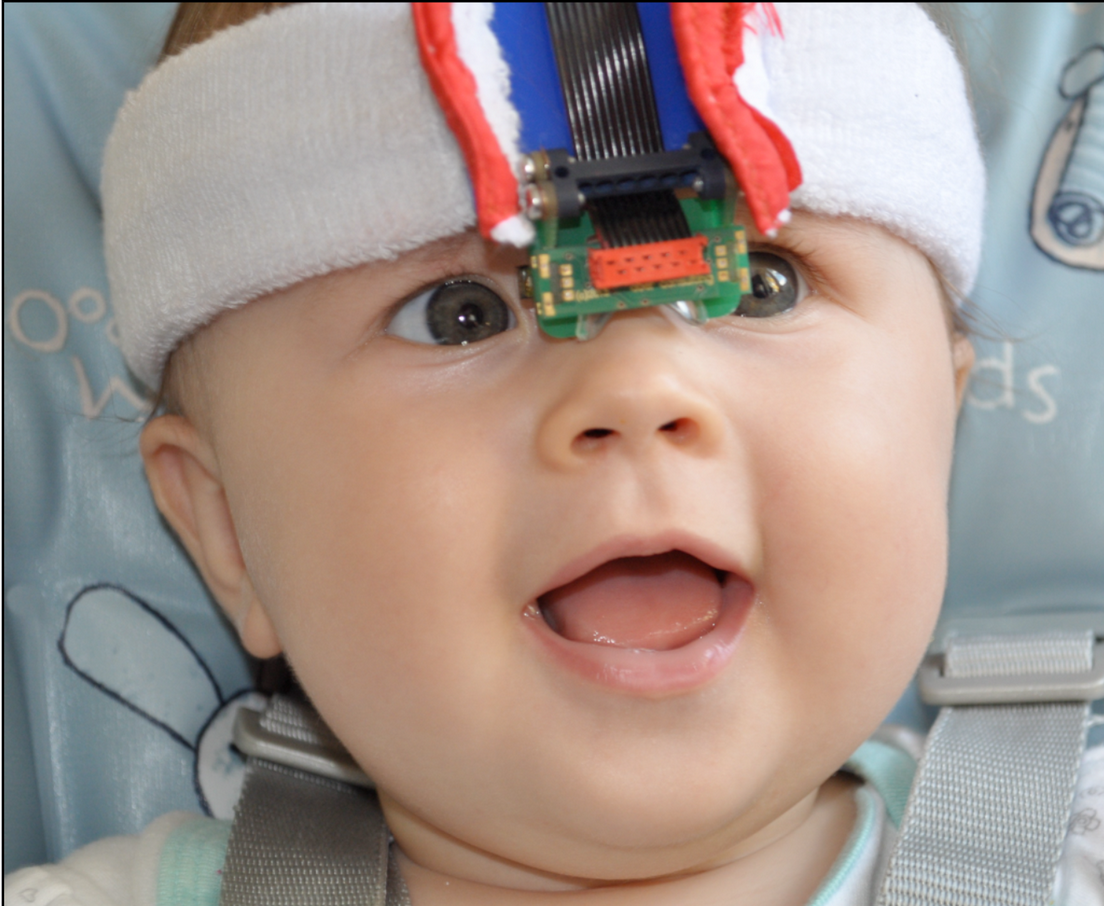
\includegraphics[width=.17\textwidth]{captor_ober}}
	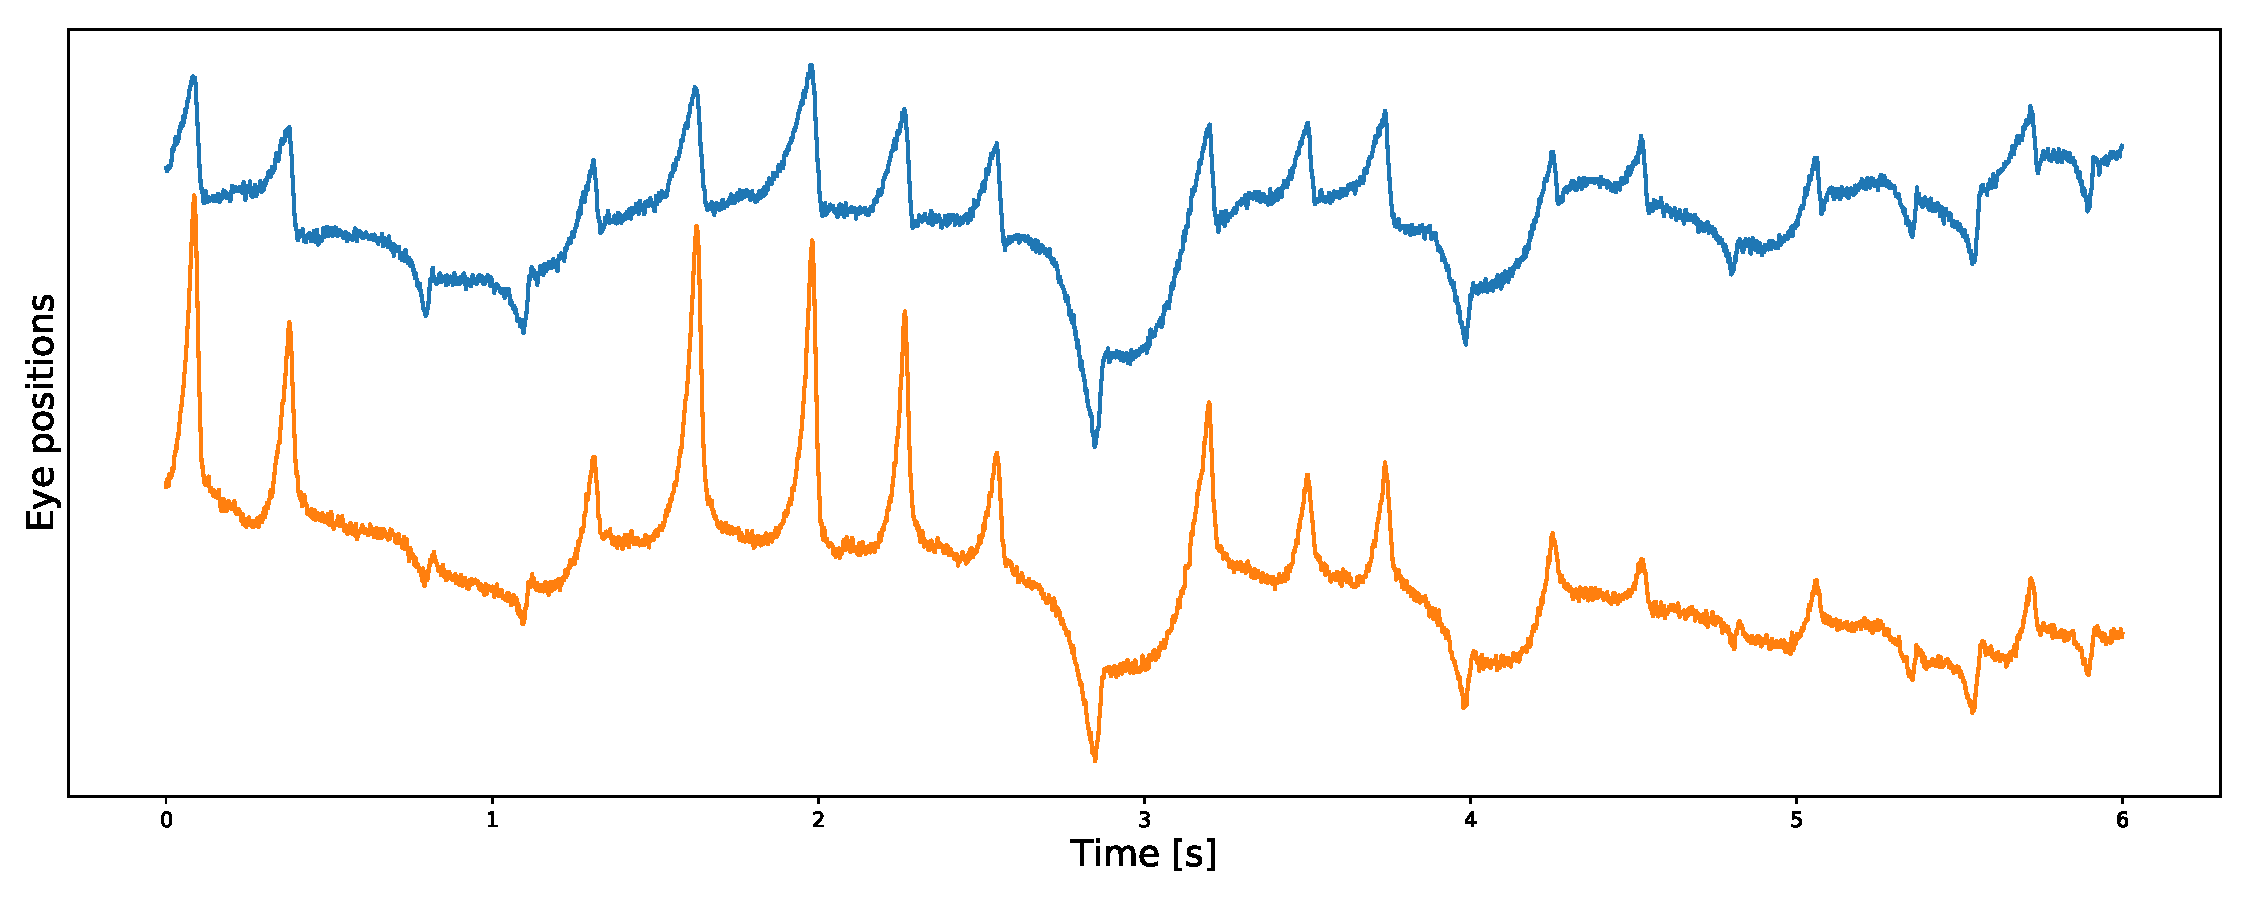
\includegraphics[width=.8\textwidth, height=7em]{oculo}\\[0em]
	\raisebox{1.5em}{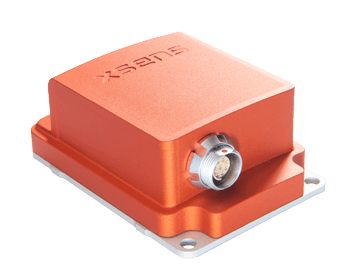
\includegraphics[width=.17\textwidth]{xsens}}
	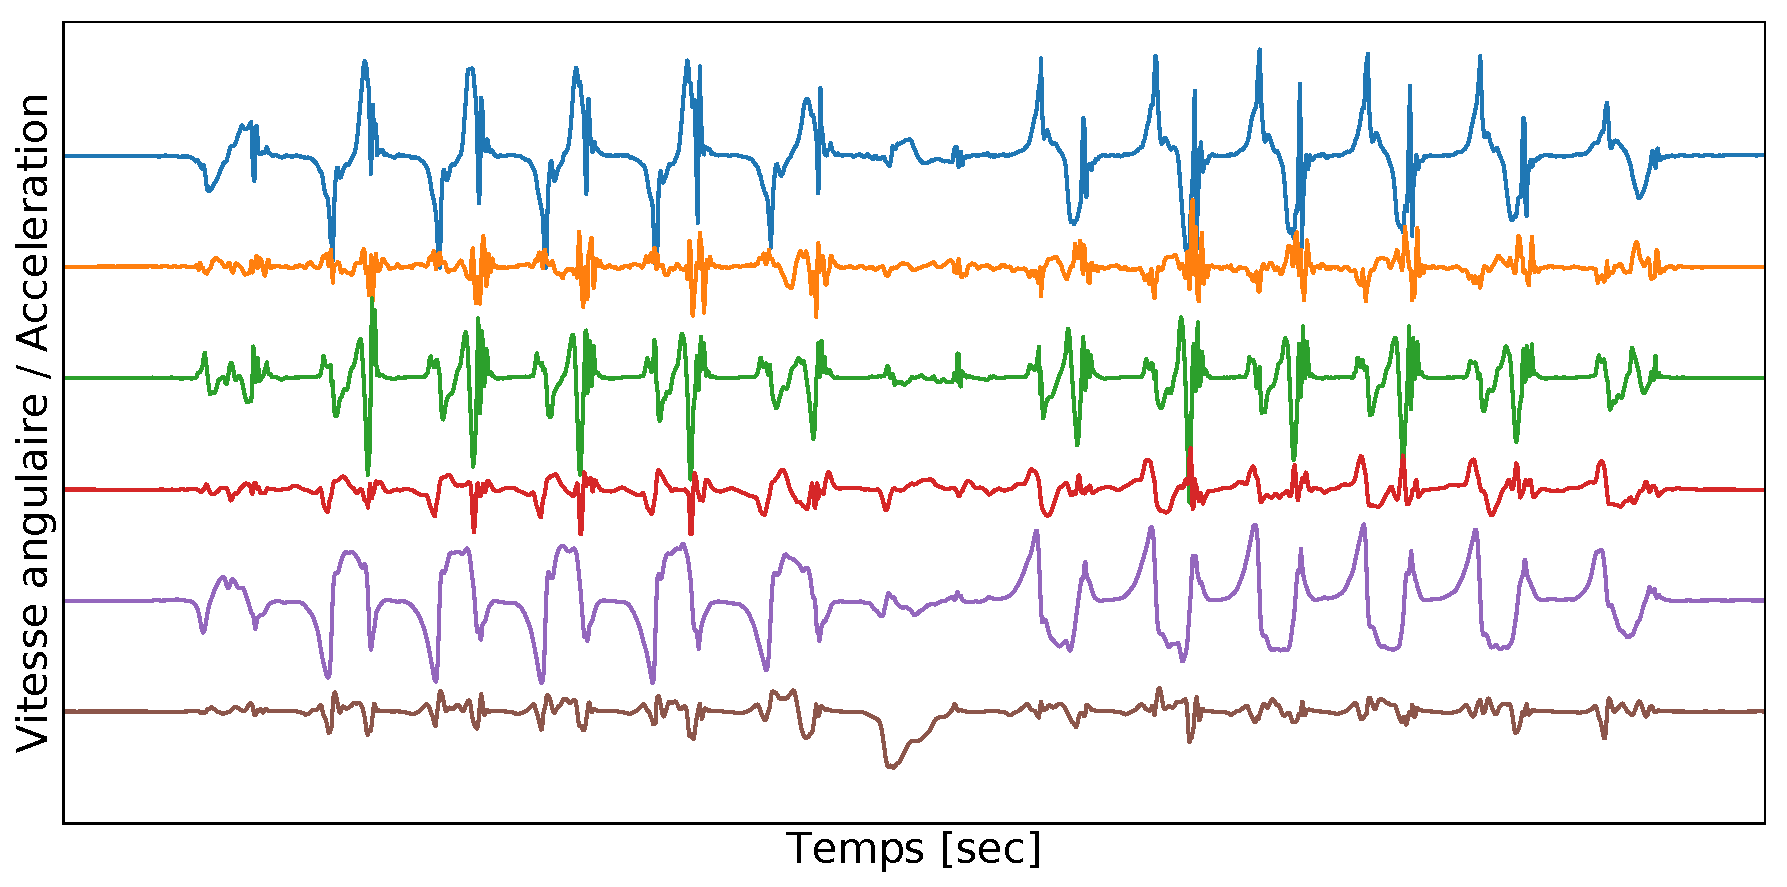
\includegraphics[width=.8\textwidth, height=7em]{accelero}\\[.2em]
	\large\textbf{Accelerometers}\\[.2em]
	\biblio{}

\end{frame}

\begin{frame}{Physiological signals}
	\large
	Studies with many constraints:\\[1em]
	\begin{itemize}\itemsep.0em
		\item Non-stationary\\\keypoint{Adaptive methods}
		\item High-dimension\\\keypoint{Scalable}
		\item High-variability\\\keypoint{Dimension reduction}
		\item Interpretability\\\keypoint{Sparsity}
	\end{itemize}
\end{frame}


\begin{frame}{Encoding a walk signal}
	\centering
	\includegraphics[width=\textwidth]{walk/csc_random}
	The activation are concentrated around the steps but there is some dispersion
	on multiple patterns.
\end{frame}

%\begin{frame}{Sparse Convolutional Representation}

%\textbf{Notation:}
%\begin{itemize}
%	\item $X$ a signal of length $T$
%	\item $\mathcal E$ is a noise signal of length $T$ 
%	\item $\pmb D$ is a set of $K$ patterns of length $W$
%	\item $Z$ is a signal of length $L = T-W+1$ in $\Rset^K$ 
%\end{itemize}
%\begin{align*}
%	X[t] & = \sum_{k=1}^K (Z_k*\pmb D_k)[t] + \mathcal E[t]\\
%		 & = \sum_{k=1}^K \sum_{\tau=0}^{W-1}Z_k[t-\tau]*\pmb D_k[\tau] + \mathcal E[t]
%\end{align*}
%\vskip.5em
%with $Z$ sparse. {\color{gray} Few of its coefficients are non-zero.}
	
%\end{frame}
\begin{frame}{Sparse Representation}

\textbf{Notation:}
\begin{itemize}
	\item $x$ a vector in $\Rset^P$
	\item $\mathcal E$ is a noise signal in $\Rset^P$  
	\item $D \in \Rset^{P\times K}$ is a set of $K$ patterns in $\Rset^P$ 
	\item $Z$ is a coding vector in $\Rset^K$ 
\end{itemize}
\vskip1em
{\bf Linear model:}
\begin{align*}
	x & = Dz + \mathcal E
\end{align*}
\vskip.5em
with $z$ sparse. {\color{gray} Few of its coefficients are non-zero.}
	
\end{frame}

\begin{frame}{Learning Sparse Representation}
Dictionary learning optimization problem
\[
	z^*, D^* = \argmin_{z, D}\frac{1}{N}\sum_{n=1}^N
			\underbrace{\| x^{[n]} - D z^{[n]}\|_2^2
						}_{\text{data fit}} +
			\underbrace{\lambda\| z^{[n]}\|_1 + \textbf{1}_{\Omega}(D)
						}_{\text{penalizations}}
\]
with a constraing set $\Omega$ and a regularization parameter $\lambda > 0$.\\[1em] 
This problem is non-convex and is generaly solved using an alternate minimization:

\begin{enumerate}\itemsep.5em
	\item \textbf{Dictionary update:} $z$ fixed, update $ D$ 
	\item \textbf{Sparse coding:} $ D$ fixed, update $Z$, independent for each $n\in\llbracket1, N\rrbracket$ 
\end{enumerate}

	
\end{frame}

\begin{frame}<presentation:0>{Sparse coding}
\begin{columns}[T]

\column{.47\textwidth}
\textbf{Convolutional LASSO}
\begin{itemize}
	\item Signal $X$
	\item Signal $Z$ in $\Rset^K$  
	\item Dictionary $\pmb D$ 
	\item Minimization
	\[
		\frac{1}{2}\| X - \sum_{k=1}^K Z_k*\pmb D_k\|_2^2+ \lambda\| Z \|_1
	\]
\end{itemize}

\column{.49\textwidth}
\textbf{LASSO}\mycite{Tibshirani1996}
\begin{itemize}
	\item Vector $x \in \Rset^T$ representing $X$ 
	\item Vector $z \in \Rset^{KL}$ representing $Z$
	\item Band circulant matrix $D$ 
	\item Minimization
	\[
		\phantom{\sum_{k=1}^K}\frac{1}{2}\| x - Dz\|_2^2+ \lambda\| z \|_1
	\]
\end{itemize}
\end{columns}
\vskip1em
\textbf{Related algorithms:}\\[.5em]
	\begin{tabular}{l p{5em} r }
%		Methods & {Original paper for sparse coding} & Convolutional adaptation\\
		FSS && \cite{Grosse2007, Lee2007} \\
		FISTA && \cite{Beck2009,Chalasani2013}\\
		ADMM && \cite{Gabay1976,Bristow2013} \\
		CD && \cite{Friedman2007,Kavukcuoglu2013} \\
	\end{tabular}

\end{frame}

\begin{frame}{Sparse coding algorithm}

\begin{itemize}\itemsep1.5em
	\item ISTA \mycite{Daubechies2004}
	\item Fast ISTA \mycite{Beck2009}
	\item ADMM \mycite{Gabay1976}
	\item Coordinate Descent \mycite{Friedman2007}
	\item Feature Sign-Search \mycite{Lee2007}
\end{itemize}
	
\end{frame}

\begin{frame}[t]{Learned Iterative Soft-Thresholding Algorithm (LISTA)}
	We have to solve $N$ problems with a common structure $D$.\\[.5em]
	{\Large\centering \textbf{Can we use this structure?}\\[.5em]}
	\only<2>{

	\begin{figure}
	\begin{subfigure}[b]{.47\textwidth}
		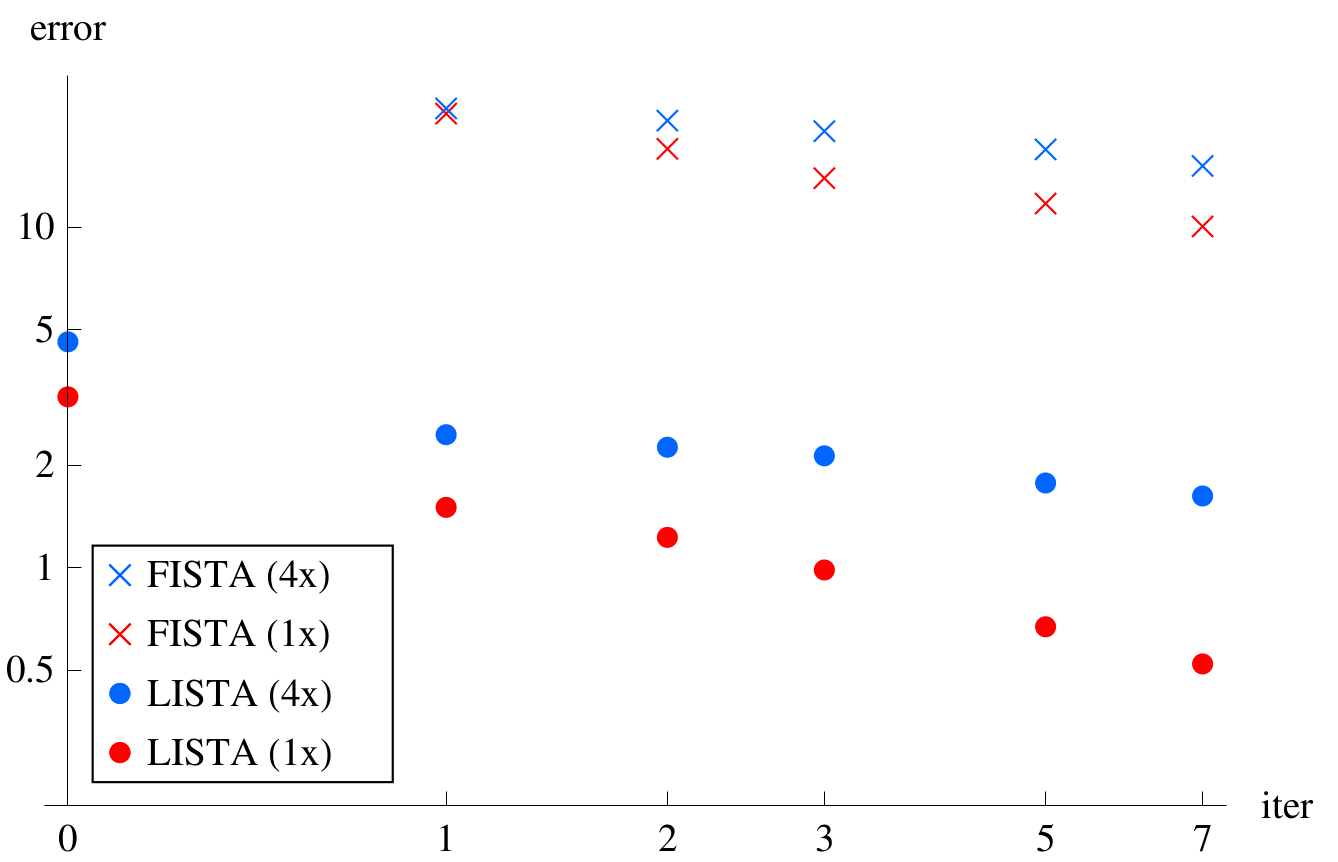
\includegraphics[width=\textwidth]{Gregor10}
	\end{subfigure}
	\begin{subfigure}[b]{.5\textwidth}
		\centering
		\inputTikZ{.8}{ista_tikz.tex}
		\inputTikZ{.6}{lista_tikz.tex}
	\end{subfigure}
	\caption*{LISTA -- Adapted from \cite{Gregor10}}
	\end{figure}\vskip-1em
	\centering
	\Large\textbf{Why does it work?}
	}
\end{frame}



\end{document}